% igs2ejournalguide.tex
% v4.00 3-sept-2015

\NeedsTeXFormat{LaTeX2e}

% check that the math fits the two-column format:
 \documentclass[twocolumn, letterpaper]{igs}

% but use this version when submitting your article:
% \documentclass[review,oneside, letterpaper]{igs}

 % \usepackage{igsnatbib}
  \usepackage{lmodern}
\usepackage{amsmath,amssymb,amsthm}
\usepackage{natbib} 
\usepackage{wrapfig}
\usepackage{enumitem}
\usepackage{multirow}
\usepackage{tabularx}
\usepackage{booktabs}

\newcolumntype{C}{>{\centering\arraybackslash}X}
\renewcommand{\tabularxcolumn}[1]{m{#1}}%


% check if we are compiling under latex or pdflatex
  \ifx\pdftexversion\undefined
    \usepackage[dvips]{graphicx}
  \else
    \usepackage[pdftex]{graphicx}
    \usepackage{epstopdf}
    \epstopdfsetup{suffix=}
  \fi


\begin{document}

\title[]{Uncertainties in estimating winter balance from direct measurements on  glaciers}

\author[]{Alexandra PULWICKI,$^1$
  Gwenn E. FLOWERS,$^1$ Valentina  RADI\'C,$^2$}

\affiliation{%
$^1$ Simon Fraser University, Burnaby, BC, Canada\\
$^2$University of British Columbia, Vancouver, BC, Canada\\
  Correspondence: Alexandra Pulwicki 
  $<$apulwick@sfu.ca$>$}


%%%%%%%%%%%%%%%%%%%%%%%%%%%%%%%%%
%	ABSTRACT
%%%%%%%%%%%%%%%%%%%%%%%%%%%%%%%%%

\abstract{Accurately estimating winter surface mass balance for a glacier is central to quantifying overall mass balance and melt runoff. However, measuring and modelling snow distribution and variability is inherently difficult in alpine terrain, resulting in high winter balance uncertainty. The goal of this paper is to examine methods and sources of error when converting snow measurements to estimates of winter balance and to gain a more comprehensive understanding of uncertainties inherent in this process. We extensively measure snow depth and density, at various spatial scales, on three glaciers in the St. Elias Mountains, Yukon. Elevation is found to be the dominant driver of accumulation variability but the relationship varies between glaciers. Our results also suggest that wind redistribution and preferential deposition affect snow distribution but that more complex parametrization is need to fully capture wind effects. By using a Monte Carlo method to quantify the effects of various sources of uncertainty, we find that interpolation of SWE measurements is the largest source of winter balance uncertainty. Snow distribution patterns differed considerably between glaciers, highlighting strong inter- and intra-basin variability. Accurately and precisely estimating winter balance therefore continues to be a difficult and elusive problem. }

\maketitle




%%%%%%%%%%%%%%%%%%%%%%%%%%%%%%%%%
%	INTRODUCTION
%%%%%%%%%%%%%%%%%%%%%%%%%%%%%%%%%
\section{Introduction}

Accurate estimation of winter surface mass balance is critical for correctly simulating the summer and overall mass balance of a glacier \citep[e.g.][]{Reveillet2016}. Effectively representing spatial distribution of snow is also important for simulating snow and ice melt as well as energy and mass exchange between the land and atmosphere to better monitor surface runoff and its downstream effects \citep[e.g.][]{Clark2011}. Snow distribution is sensitive to a number of complex process that partially depend on glacier location, topography, and orientation \citep[e.g.][]{Bloschl1991, Mott2008, Clark2011, Sold2013}. Current models are not able to fully represent these processes so the distribution of snow in remote, mountainous locations is not well known. There is, therefore, a significant source of uncertainty that undermines the ability of models to represent current glacier conditions and make predictions of glacier response to a warming climate \citep{Reveillet2016}. 

Winter surface mass balance is the net accumulation and ablation of snow over the winter season \citep{Cogley2011}, which constitutes glacier mass input. We refer to this quantity as winter balance throughout the paper. Accurate estimates of winter balance are critical for calculating glacier mass balance, not only because winter balance constitutes half of the glacier mass balance but also because the distribution of snow on a glacier initializes the summer balance and high snow albedo contributes to reduced summer melt \citep[e.g.][]{Hock2005, Reveillet2016}. 

Winter balance is notoriously difficult to estimate. Snow distribution in alpine regions is highly variable and influenced by dynamic interactions between the atmosphere and complex topography, operating on multiple spatial and temporal scales \citep[e.g.][]{Barry1992, Liston2006, Clark2011}. Extensive, high resolution and accurate accumulation measurements on glaciers are almost impossible to achieve due to cost benefits of the various methods used to quantify snow water equivalent \citep[e.g.][]{Cogley2011, McGrath2015}. For example, snow probes obtain accurate point observations but have negligible spatial coverage. Conversely, gravimetric methods obtain extensive measurements of mass change but cannot capture relevant spatial variability of snow \citep{Cogley2011}. Glacierized regions are also generally remote and challenging to access during the winter due to poor travelling conditions. 

Most glacier mass balance programs estimate winter balance in a similar way to summer balance. Measurements of the amount of snow at the end of the winter season are taken at a few stake locations and then basic interpolation methods are used to estimate winter balance \citep[e.g.][]{Hock1999, Thibert2008, MacDougall2011, Cullen2017}. However, equivalence between summer and winter balance estimation methods is likely inappropriate. Melt is strongly affected by air temperature and solar radiation \citep[e.g.][]{Hock2005}, both of which are consistent across large spatial domains \citep[e.g.][]{Barry1992}. Conversely, snow distribution is largely driven by precipitation \citep[e.g.][]{Lehning2008} and wind patterns \citep[e.g.][]{Bernhardt2009, Musselman2015}, which are known to be highly heterogeneous in alpine environments \citep[e.g.][]{Barry1992}. Snow distribution is therefore highly variable and has short correlation length scales \citep[e.g.][]{Anderton2004, Egli2011, Grunewald2010, Helbig2017, Lopez2011, Lopez2013, Machguth2006, Marshall2006}. 

Detailed studies of winter balance are far less common than those of summer balance and uncertainty in winter mass balance currently overshadows differences between summer balance models \citep[e.g.][]{Reveillet2016}. Studies that focus on estimating winter balance employ a wide range of snow measurement techniques \citep{Sold2013}, including direct measurement \citep[e.g.][]{Cullen2017}, lidar/photogrammerty \citep[e.g.][]{Sold2013} and ground penetrating radar \citep[e.g.][]{Machguth2006, Gusmeroli2014, McGrath2015}. Spatial coverage of measurements is often limited for winter balance studies and typically consists of an elevation transect along the glacier centreline \citep[e.g.][]{Kaser2003, Machguth2006}. Interpolation of these measurements is primarily done by computing a linear regression that includes only a few topographic parameters \citep[e.g.][]{MacDougall2011}, with elevation being the most common. Other applied techniques include hand contouring \citep[e.g.][]{Tangborn1975}, kriging \citep[e.g.][]{Hock1999} and attributing measured accumulation values to elevation bands \citep[e.g.][]{Thibert2008}. Physical snow models have been applied on a few glaciers \citep[e.g.][]{Mott2008, Dadic2010} but a lack of detailed meteorological data generally prohibits their wide-spread application. Error analysis is rarely considered and to our knowledge, no studies have investigated uncertainty in winter balance estimates. 

There is a disparity in snow survey sophistication within glacier winter balance studies when compared to snow science studies. Winter mass balance surveys employ similar techniques and methods as snow science surveys \citep[e.g.][]{Elder1991,Deems2006, Nolan2015,Godio2016} but favour more simple approaches \citep[e.g.][]{Kaser2003, Sold2013}. Snow science surveys are generally extensive and designed to measure snow throughout the basin and ensure that all terrain types are sampled. A wide array of measurement interpolation methods are used, including linear \citep[e.g.][]{Lopez2010} and non-linear regressions \citep[e.g.][]{Molotch2005} and geospatial interpolation \citep[e.g.][]{Erxleben2002} such as kriging, and methods are often combined to yield improved fit \citep[e.g.][]{Balk2000}. Physical snow models, such as Alpine3D \citep{Lehning2006} and SnowDrift3D \citep{Schneiderbauer2011}, are continuously being improved and tested within the snow science literature. Snow survey error has been considered from both a theoretical \citep[e.g.][]{Trujillo2015} and applied perspective \citep[e.g.][]{Turcan1975,Woo1978, Deems2006}. 

The precision and accuracy of winter balance estimates can likely be improved by incorporating snow science tools and interpolation methodologies and by gaining a more comprehensive understanding of uncertainties inherent when estimating winter balance on glaciers. Ultimately, we need a thorough knowledge of the processes that affect spatial and temporal snow variability and an effective method to predict snow accumulation. The contribution of our work toward these goals is to (1) examine methods and uncertainties when moving from direct snow depth and density measurements to estimating winter balance and (2) show how snow variability, data error and our methodological choices interact to create uncertainty in our estimate of winter balance. We focus on commonly applied low-complexity methods of measuring and predicting winter balance with the hope of making our results broadly applicable to current and future winter mass balance programs.


%%%%%%%%%%%%%%%%%%%%%%%%%%%%%%%%%
%	STUDY SITE
%%%%%%%%%%%%%%%%%%%%%%%%%%%%%%%%%

\section{Study site}

Winter balance surveys were conducted on three glaciers in the Donjek Range of the St. Elias Mountains, located in the south western Yukon, Canada. The Donjek Range is approximately $30\times30$ km and Glacier 4, Glacier 2, and Glacier 13 (labelling adopted from \cite{Crompton2016}) are located along a SW-NE transect through the range. There is a local topographic divide in the Donjek Range that follows an ``L'' shape, with one glacier located in each of the south, north, and east regions (Figure \ref{fig:Sampling}). These mid-sized alpine glaciers are generally oriented SE-NW, with Glacier 4 dominantly south facing and Glaciers 2 and 13 generally north facing. The glaciers are low angled with steep head walls and steep valley walls. The St. Elias mountains boarder the Pacific Ocean and rise sharply, creating a significant climatic winter gradient between coastal maritime conditions, generated by Aleutian--Gulf of Alaska low-pressure systems, and interior continental conditions, determined by Yukon--Mackenzie high-pressure system \citep{Taylor1969}. The average dividing line between the two climatic zones shifts between Divide Station and the head of the Kaskawalsh Glacier based on synoptic conditions. The Donjek Range is located approximately 40 km to the east of the head of the Kaskawalsh Glacier. Research on snow distribution and glacier mass balance in the St. Elias is limited. A series of research programs were operational in the 1960s \citep{Wood1948, Danby2003} and long-term studies on a few alpine glaciers have arisen in the last 30 years \citep[e.g.][]{Clarke1984, Paoli2009}.

\begin{table*}[]
\centering
\caption{Physical details of study glaciers as well as details of snow survey conducted in May 2016 at Glacier 4 (G4), Glacier 2 (G2), and Glacier 13 (G13). Values shown include number of snow depth measurement locations along transects ($n_{\mathrm{T}}$), total length of transects ($d_{\mathrm{T}}$ [km]), number of combined SP and FS density measurement locations ($n_{\rho}$) and number of zigzag ($n_{\mathrm{zz}}$).}
\label{tab:GlacierDetails}
\begin{tabular}{ccccccccccc}
\midrule
\textbf{} & \multirow{2}{*}{\textbf{Location}} & \multicolumn{2}{c}{\textbf{Elevation (m a.s.l)}} & \textbf{Slope ($^{\circ}$)} & \multirow{2}{*}{\textbf{\begin{tabular}[c]{@{}c@{}}Area\\ (km)\end{tabular}}} & \multicolumn{5}{c}{\textbf{Survey Details}} \\
 &  & \textit{Mean} & \textit{Range} & \textit{Mean} &  & \textit{Date} & $n_{\mathrm{T}}$ & $d_{\mathrm{T}}$ (km) & $n_{\rho}$ & $n_{\mathrm{zz}}$ \\ \midrule
\textbf{G4} & \begin{tabular}[c]{@{}c@{}}595470 E\\ 6740730 N\end{tabular} & 2344 & 1958--2809 & 12.8 & 3.8 & May 4--7 & 649 & 13.1 & 7 & 3 \\
\textbf{G2} & \begin{tabular}[c]{@{}c@{}}601160 E\\ 6753785 N\end{tabular} & 2495 & 1899--3103 & 13.0 & 7.0 & May 8--11 & 762 & 13.6 & 7 & 3 \\
\textbf{G13} & \begin{tabular}[c]{@{}c@{}}604602 E\\ 6763400 N\end{tabular} & 2428 & 1923--3067 & 13.4 & 12.6 & May 12--15 & 941 & 18.1 & 19 & 4
\end{tabular}
\end{table*}

%%%%%%%%%%%%%%%%%%%%%%%%%%%%%%%%%
%	METHODS
%%%%%%%%%%%%%%%%%%%%%%%%%%%%%%%%%


\section{Methods}

Estimating winter balance involves transforming snow depth and density measurements to distributed estimates of snow water equivalent (SWE). We use four main processing steps. First, we obtain measurements of snow depth and density. Since density is measured more sparsely than depth, the second step is to interpolate density measurements to all depth measurement locations and to calculate the SWE at each measurement location. Third, we average all SWE values within one grid cell of a digital elevation model (DEM) with given spatial resolution to produce a single value of SWE for each grid cell. Fourth, we interpolate SWE values to obtain a distributed estimate of SWE across the surface of the glacier. We choose to use a linear regression between SWE and topographic parameters as well as simple kriging to interpolation grid cell SWE. To estimate the specific winter balance we then calculate aerially-averaged integrated SWE. For brevity, we refer to these four steps as (1) field measurements, (2) distributed snow density, (3) grid cell average SWE and (4) distributed SWE. Detailed methodology for each step is outlined below.

\subsection{Field measurements}

\begin{figure*}
	\centering
	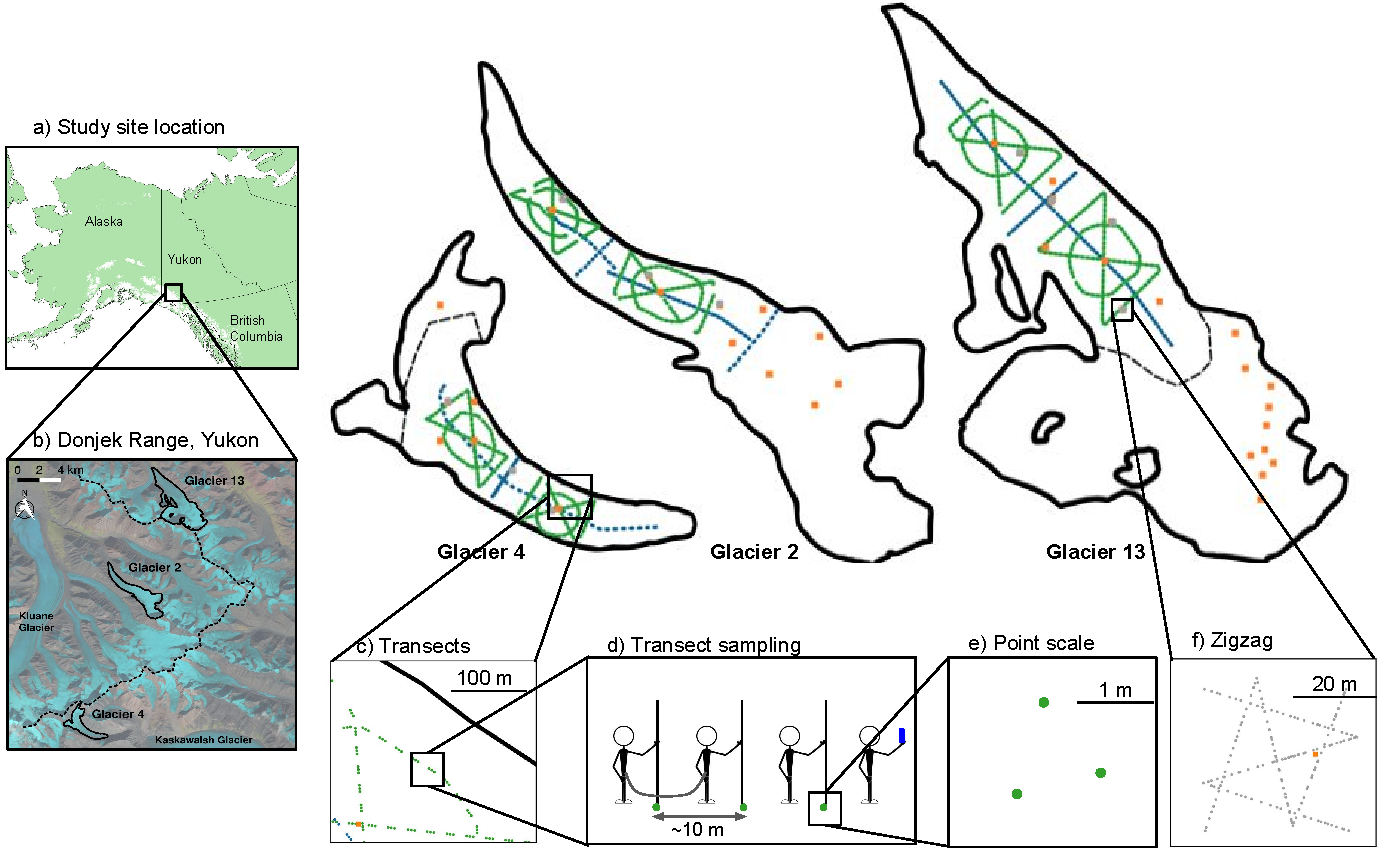
\includegraphics[width =\textwidth]{Sampling.pdf}\\
	\caption{Sampling design for Glaciers 4, 2 and 13, located in the Donjek Range, Yukon (a,b). Centreline and transverse transects are shown in blue dots, hourglass and circle design are shown in green dots. (c) Linear and curvilinear transects typically consist of sets of three measurement locations, spaced $\sim$10 m apart (d). (e) At each measurement location, three snow depth observation are made. (f) Linear-random snow depth measurements in `zigzag' design are shown as grey dots. Orange squares are locations of snow density measurements. }
	\label{fig:Sampling}
\end{figure*}

\subsubsection{Sampling design}

The sampling design attempted to capture depth variability at multiple spatial scales. We measured winter balance at three glaciers along the precipitation gradient in the St. Elias Mountains, Yukon \citep{Taylor1969} in an attempt to account for range-scale variability \citep{Clark2011}. We measured winter balance on Glaciers 4, 2, and 13, which are located increasingly far from the head of the Kaskawalsh Glacier (Figure \ref{fig:Sampling}b). Snow depth was measured along linear and curvilinear transects to account for basin-scale variability. At each measurement location, three values of snow depth were recorded to account for point-scale variability \citep{Clark2011}.  We selected centreline and transverse transects with sample spacing of $10-60$ m (Figure \ref{fig:Sampling}d) to capture previously established correlations between elevation and accumulation \citep[e.g.][]{Machguth2006, Walmsley2015} as well as accumulation differences between ice-marginal and centre accumulation. We also implemented an hourglass and circle design (Figure \ref{fig:Sampling}), which allows for sampling in all directions and easy travel (Parr, C., 2016 personal communication). At each measurement location, we took $3-4$ depth measurements within $\sim$1 m of each other (Figure \ref{fig:Sampling}e), resulting in more than 9,000 snow depth measurements throughout the study area. 

\subsubsection{Snow depth}

The estimated SWE is the product of the snow depth and depth-averaged density. Snow depth is generally accepted to be more variable than density \citep{Elder1991, Clark2011, Lopez2013} so we chose a sampling design with relatively small measurement spacing along transects that resulted in a ratio of approximately 55:1 snow depth to snow density measurements. Our sampling campaign involved four people and occurred between May 5 and 15, 2015, which corresponds to the historical peak accumulation in the Yukon (Yukon Snow Survey Bulletin and Water Supply Forecast, May 1, 2016). While roped-up for glacier travel at fixed distances between observers, the lead person used a single frequency GPS (Garmin GPSMAP 64s) to navigate as close to the predefined transect measurement locations as possible (Figure \ref{fig:Sampling}). The remaining three people used 3.2 m aluminium avalanche probes to take snow depth measurements. The location of each set of depth measurements, taken by the second, third and fourth observers, was approximated based on the recorded location of the first person. 

Snow depth sampling was primarily done in the ablation area to ensure that only snow from the current accumulation season was measured. Determining the boundary between snow and firn in the accumulation area, especially when using an avalanche probe, is difficult and often incorrect \citep{Grunewald2010,Sold2013}. We intended to use a firn corer to extract snow cores in the accumulation area but due to environmental conditions we were unable to obtain cohesive cores. Successful measurements within the accumulation area were done either in a snow pit or using a Federal Sampler with shovel validation so that we could identify the snow-firn transition based on a change in snow crystal size and density. 

\subsubsection{Zigzags}

To capture variability at spatial scales smaller than a DEM grid cell, we implemented a linear-random sampling design, termed `zigzag' \citep{Shea2010}. We measured depth at random intervals ($0.3 - 3.0$ m) along two `Z'-shaped transects within three to four $40\times40$ m squares (Figure \ref{fig:Sampling}c) resulting in $135-191$ measurement points for each zigzag. Zigzag locations were randomly chosen within the upper ($\sim$2350 m a.s.l.), middle ($\sim$2250 m a.s.l.), and lower portions ($\sim$2150 m a.s.l.) of the ablation area of each glacier. We were able to measure a fourth zigzag on Glacier 13 that was located in the middle ablation area ($\sim$2200 m a.s.l.).

\subsubsection{Snow density}

Snow density was measured using a wedge cutter in three snowpits on each glacier. We measured a vertical density profile by inserting a $5\times10\times 10$ cm wedge-shaped cutter (250 cm$^3$) in 5 cm increments to extract snow samples and then weighed the samples with a spring scale \citep[e.g.][]{Gray1981,Fierz2009}. Uncertainty in estimating density from snow pits stems from measurement errors and incorrect assignment of density to layers that could not be sampled (i.e. ice lenses and `hard' layers). 

While snow pits provide the most accurate measure of snow density, digging and sampling a snow pit is time and labour intensive. Therefore, a Federal Snow Sampler (FS) \citep{Clyde1932}, which measures bulk SWE, was used to augment the spatial extent of density measurements. A minimum of three measurements were taken at each of $7-19$ locations on each glacier and an additional eight FS measurements were co-located with each snow pit profile. Measurements where the snow core length inside the FS was less than 90\% of the snow depth were assumed to be an incorrect sample and were excluded. Density values were then averaged for each location. 

During the field campaign there were two small accumulation events. The first, on May 6, also involved high winds so accumulation could not be determined. The second, on May 10, resulted in 0.01 m w.e accumulation at one location on Glacier 2. Warm temperatures and clear skies occurred between May 11 and 16, which we believed resulted in significant melt occurring on Glacier 13. The snow in the lower part of the ablation area was isothermal and showed clear signs of melt and snow metamorphosis. The total amount of accumulation and melt during the study period could not be estimated so no corrections were made. 

\subsection{Distributed snow density}

Measured density is interpolated to estimate SWE at each depth sampling location. We chose four separate methods that are commonly applied to interpolate density: (1) mean density over an entire range \citep[e.g.][]{Cullen2017}, (2) mean density for each glacier \citep[e.g.][]{Elder1991, McGrath2015}, (3) linear regression of density with elevation \citep[e.g.][]{Elder1998, Molotch2005} and (4) inverse-distance weighted density \citep[e.g.][]{Molotch2005}.  SP and FS densities are treated separately, for reasons explained below, which results in eight density interpolation options (Table \ref{tab:densityOptions}).

\begin{table}
\centering
\caption{Description of density interpolation methods used to calculate SWE used in the topographic regression. Abbreviations with `S' used snowpit-derived densities and abbreviations with an `F' used Federal Sampler-derived densities.}
\label{tab:densityOptions}
\begin{tabular}{cccc}
\midrule
 & \multicolumn{2}{c}{\textbf{Snow density source}} &  \\
 & \textit{Snowpit} & \begin{tabular}[c]{c} \textit{Federal}\\  \textit{Sampler}\end{tabular} & \multirow{-2}{*}{\textbf{\begin{tabular}[c]{c}Estimation\\ method\end{tabular}}} \\   \midrule
S1 & $\blacksquare$ &  &  \\
F1 &  & $\blacksquare$ & \multirow{-2}{*}{\begin{tabular}[c]{@{}c@{}}Mean of all glaciers \end{tabular}} \\  \midrule
S2 & $\blacksquare$ &  &  \\
F2 &  & $\blacksquare$ & \multirow{-2}{*}{Glacier mean} \\ \midrule
S3 & $\blacksquare$ &  &  \\
F3 &  & $\blacksquare$ & \multirow{-2}{*}{\begin{tabular}[c]{@{}c@{}}Linear regression of elevation \\ and density for each glacier \end{tabular}} \\ \midrule
S4 & $\blacksquare$ &  &  \\
F4 &  & $\blacksquare$ & \multirow{-2}{*}{\begin{tabular}[c]{@{}c@{}}Inverse distance\\ weighted mean\end{tabular}}
\end{tabular}
\end{table}
 

\subsection{Grid cell average SWE}

We average SWE values within each DEM-aligned grid cell ($40 \times 40$ m). The locations of measurements have considerable uncertainty both from the error of the GPS unit ($2.7 - 4.6$ m) and the estimation of observer location based on the GPS unit. These errors could easily result in the incorrect assignment of a SWE measurement to a certain grid cell but this source of variability was not further investigated because we assume that SWE variability is captured in the zigzag measurements described below. There are no significant differences between observers (p$>$0.05), with the exception of the first transect on Glacier 4. No corrections to the data based on observer differences are applied.

\subsection{Distributed SWE}

\subsubsection{Linear regression}

SWE are interpolated and extrapolated for each glacier using linear regression (LR) as well as simple kriging (SK). Linear regressions relate observed SWE to grid cell values of DEM-derived topographic parameters \citep{Davis1986}. We choose to include elevation, distance from centreline, slope, aspect, curvature, ``northness'' and a wind redistribution parameter in the LR. For details on data and methods used to estimate the topographic parameters see the Supplementary Material. Topographic parameters are weighted by a set of fitted regression coefficients ($\beta_i$). Regression coefficients are calculated by minimizing the sum of squares of the vertical deviations of each data point from the regression line \citep{Davis1986}. Snow depth data are highly variable so there is a possibility for the LR to fit to this data noise, a process known as overfitting. To prevent overfitting, cross-validation and model averaging are implemented (see Supplementary Material). The distributed estimate of SWE is found by using regression coefficients to estimate SWE at each grid cell. Specific winter balance is calculated as the aerially-averaged, integrated SWE for each glacier ([m w.e.]). 

\subsubsection{Simple kriging}

Simple kriging (SK) estimates SWE values at unsampled locations by using the isotropic spatial correlation (covariance) of measured SWE to find a set of optimal weights \citep{Davis1986, Li2008}. SK assumes that if sampling points are distributed throughout a surface, the degree of spatial correlation of the observed surface can be determined and the surface can then be interpolated between sampling points. We used the \texttt{DiceKriging} R package \citep{Roustant2012} to calculate the maximum likelihood covariance matrix, as well as range distance ($\theta$) and nugget. The range distance is a measure of data correlation length and the nugget is the residual that encompasses sampling-error variance as well as the spatial variance at distances less than the minimum sample spacing \citep{Li2008}. 

\subsection{Uncertainty analysis}

To quantify effects of uncertainty on the winter balance estimate, we conduct a Monte Carlo experiment, which uses repeated random sampling to calculate a numerical solution \citep{Metropolis1949}. This random sampling process is done 1000 times, which results in a distribution of possible winter balance values based on uncertainty within the data processing steps. We quantify the effect of uncertainty as the standard deviation of the distribution. Three sources of uncertainty, which encompass error and uncertainty within each processing step, are considered: (1) density uncertainty, (2) SWE uncertainty and (3) interpolation uncertainty. Individual sources of uncertainty are propagated through the process of converting snow measurements to winter balance. Then, all three uncertainty sources are considered together and their combined effect on winter balance uncertainty is quantified.

	\subsubsection{SWE uncertainty ($\sigma_{\mathrm{SWE}}$)}
To estimate winter balance, we must represent SWE within a grid cell with a single value despite the fact that each grid cell contains a distribution of SWE values. The resulting uncertainty from this SWE representation is characterized by generating a normal distribution, with a standard deviation equal to the mean standard deviation of all zigzags on each glacier. For each iteration of the Monte Carlo, a set of random values is generated from the distribution and added to the observed SWE values. These perturbed SWE values are then used to estimate winter balance. The winter balance uncertainty due to SWE uncertainty ($\sigma_{\mathrm{SWE}}$) is calculated as the standard deviation of the resulting distribution of winter balance estimates.  

	\subsubsection{Density uncertainty ($\sigma_{\rho}$)}
We incorporate uncertainty in interpolating density measurements by carrying forward all eight density interpolation options when estimating winter balance. The density measurement and interpolation methods used in our study encompass a broad spectrum of possible density values. The winter balance uncertainty due to density uncertainty ($\sigma_{\rho}$) is calculated as the standard deviation of winter balance estimates calculated using each density interpolation option.

	\subsubsection{Interpolation uncertainty ($\sigma_{\mathrm{INT}}$)}
We represent the uncertainty in fitting an interpolation model to observed data in different ways for LR and SK. LR uncertainty is represented by obtaining a multivariate normal distribution of possible $\beta_i$ values. The standard deviation of each distribution is calculated using the covariance of regression coefficients as outlined in \cite{Bagos2015}. The $\beta_i$ distributions are randomly sampled and the new $\beta_i$ values are used to estimate winter balance. SK uncertainty is derived from the 95\% confidence interval SWE surfaces generated within the \texttt{DiceKriging} package. The standard deviation of each grid cell is then calculated from the confidence interval surfaces and the glacier wide standard deviation is found by taking the square root of the average variance. The distribution of winter balance values is centred at the SK winter balance estimate and has a standard deviation equal to the glacier wide standard deviation. For consistency, the standard deviation of winter balance values that result from either LR or SK interpolation uncertainty is referred to as $\sigma_{\mathrm{INT}}$.



%%%%%%%%%%%%%%%%%%%%%%%%%%%%%%%%%%%%%%%%%%%
%%  RESULTS AND DISCUSSION
%%%%%%%%%%%%%%%%%%%%%%%%%%%%%%%%%%%%%%%%%%%
\section{Results and Discussion}

\subsection{Field measurements}

\begin{figure*}
	\centering
	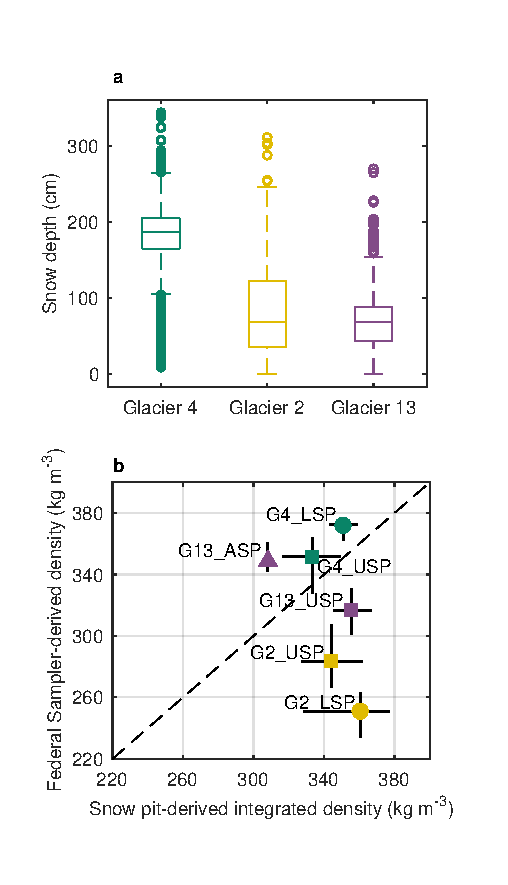
\includegraphics[width =\textwidth]{DepthBoxplot_SPvsFS.pdf}\\
	\caption{(Left) Boxplot of measured snow depth on Glaciers 4, 2 and 13. The box shows first quartiles, the line within the box indicates data median, bars indicate minimum and maximum values (excluding outliers), and circles show outliers, which are defined as being outside of the range of 1.5 times the quartiles (approximately $\pm2.7\sigma$). (Right) Comparison of integrated density estimated using wedge cutters in a snow pit and density estimated using Federal Sampler measurements for Glacier 4 (G04), Glacier 2 (G02) and Glacier 13 (G13). Snow pits were distributed in the accumulation area (ASP), upper ablation area (USP) and lower ablation area (LSP). Error bars are minimum and maximum values.}
	\label{fig:DepthBoxplot_SPvsFS}
\end{figure*}

Despite the lack of measurements in the accumulation area, especially along steep head walls, we observed a wide range of snow depth on all three study glaciers (Figure \ref{fig:DepthBoxplot_SPvsFS}). Glacier 4 has the highest mean snow depth and a high proportion of outliers, indicating a more variable snow depth overall. Glacier 13 has the lowest mean snow depth and a narrower distribution of observed values. At each measurement location, the median range of measured depths ($3-4$ points) as a percent of the mean depth at that location is 2\%, 11\%, and 12\%, for Glaciers 4, 2 and 13, respectively. 

Mean snow pit (SP) and Federal Sampler (FS) density values are within one standard deviation of each other for each glacier and over all three glaciers. The standard deviation of glacier-wide mean density is less than 10\% of the mean density. However, FS densities have a larger range of values ($227-431$kg m$^{-3}$) when compared to SP densities ($299-381$kg m$^{-3}$).  The mean SP densities are within one standard deviation between glaciers, whereas mean FS densities are not. FS and SP measurements are not correlated, while FS density values are positively correlated with snow depth. This positive relationship could be a result of physical processes, such as compaction, but is more likely a result of measurement artefacts for a number of reasons. First, the range of densities measured by the Federal sampler is large and the extreme values seem unlikely to exist in our study
region, which experiences a continental snow pack with minimal mid-winter melt events. Second, compaction effects would likely be small at these study glaciers because of the relatively shallow snow pack (deepest measurement was 340 cm). Third, no linear relationship exists between depth and SP density (R$^2 = 0.05$). Together, these findings indicate that the FS measurements have a bias which is challenging to correct for.

Uncertainty in SP density is largely due to sampling error of exceptionally dense snow layers. We quantify this uncertainty by varying three values. Ice layer density is varied between 700 and 900 kg m$^{-3}$, ice layer thickness is varied by $\pm$1 cm of the recorded thickness, and the density of layers identified as being too hard to sample (but not ice) is varied between 600 and 700 kg m$^{-3}$. The range of integrated density values is always less than 15\% of the reference density, with the largest ranges present on Glacier 2. Density values for shallow pits that contain ice lenses are particularly sensitive to changes in density and ice lens thickness. 


The FS appears to oversample in deep snow and undersample in shallow snow. Oversampling by small diameter (area of 10--12 cm$^2$) sampling tubes has been observed in previous studies, with a percent error between +6.8\% and 11.8\% \citep{Work1965, Fames1982, Conger2009}. Studies that use Federal Samplers often apply a 10\% correction to all measurements \citep[e.g.][]{Molotch2005}. Oversampling has been attributed to slots ?shaving? snow into the tube as it is rotated  \citep[e.g.][]{Dixon2012}, and to snow falling into the greater area of slots only when snow samples had densities greater than 400 kg m$^{-3}$ and snow depth greater than 1 m \citep[e.g.][]{Beaumont1963}. Undersampling is likely to occur due to snow falling out of the bottom of the sampler \citep{Turcan1975}, which likely occurred in our study since a large portion of the lower elevation snow on both Glaciers 2 and 13 was melt affected and thin, allowing for easier lateral displacement of the snow as the sampler was extracted. For example, on Glacier 13 the snow surface had been affected by radiation melt (especially at lower elevations where the snow was shallower), causing the surface to collapse when the sampler was inserted into the snow. Relatively poor scale sensitivity also made it difficult to obtain accurate measurements of small snow quantities.

\subsection{Distributed density}

Since we find no correlation between co-located SP and FS densities (Figure \ref{fig:DepthBoxplot_SPvsFS}), each set of density values is used for all four density interpolation options. Regional and glacier mean densities are higher when SP densities are used (Table \ref{tab:Density}). Density gradient with elevation differs between SP and FS densities (Table \ref{tab:Density}). At Glaciers 2 and 13, SP density decreases with elevation, likely indicating melt and/or compaction at lower elevations. SP density is independent of elevation on Glacier 4. FS density increases with elevation on Glacier 2 and there is no relationship with elevation on Glaciers 4 and 13. There is a positive linear relation (R$^2= 0.59$, p$<$0.01) between measured snow density and depth for all FS measurements. No correlation exists between SP density and elevation. Considering these results, our preferred density interpolation methods, out of four different methods we tested, is a glacier-wide mean of SP densities. Many winter balance studies assume uniform density \citep[e.g.][]{Elder1991,McGrath2015,Cullen2017} and it is realistic for future studies to measure snow density profiles at a few locations in the study basin.

\subsection{Grid cell average}

The zigzag sampling scheme offers a relatively easy way to take a large number of probe measurements in order to capture spatial variability of SWE in a grid cell. Each measured grid cell contains one to six measurements which are then averaged to give SWE grid cell average. The distribution of grid-cell SWE values for each glacier is similar to that of Figure \ref{fig:DepthBoxplot_SPvsFS} but with fewer outliers. The grid cell variability appeared to be captured with dense sampling in select grid cells but the basin-scale variability was not captured because sampling was limited to the ablation area. By decreasing transect spacing, grid cells would only have one or two measurements but more grid cells could be measured.

	%tie this into the grid cell average better %%%%%%%%%%%%%%%%%%
SWE measurements for each zigzag are not normally distributed about the mean SWE (Figure \ref{fig:ZigzagHistogram}). The average standard deviation of all zigzags on Glacier 4 is $\sigma_{\mathrm{G4}} =  0.027$ m w.e., on Glacier 2 is $\sigma_{\mathrm{G2}} =  0.035$ m w.e. and on Glacier 13 is $\sigma_{\mathrm{G13}} =  0.040$ m w.e.
	%% 

\begin{figure}
	\centering
	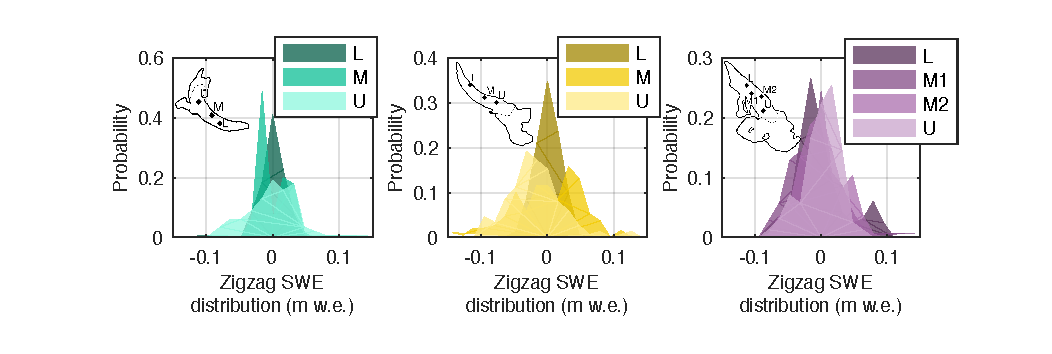
\includegraphics[width =0.5\textwidth]{ZigzagHistogram.pdf}\\
	\caption{Distribution of zigzag SWE values with the local mean subtracted on Glacier 4 (upper panel), Glacier 2 (middle panel) and Glacier 13 (lower panel). Zigzags are distributed throughout the ablation area of each glacier, with one located in the lower portion (L), one in the middle portion (M), and one in the upper portion (U). There were two zigzags in the middle ablation area of Glacier 13.}
	\label{fig:ZigzagHistogram}
\end{figure}

\subsection{Interpolated SWE}
 
The choice of interpolation method affects the specific winter balance (Table \ref{tab:WSMB&RMSE}). SK produces the highest winter balance on Glacier 4 and the lowest winter balance on Glacier 13. winter balance estimated by SK is $\sim$30\% lower than winter balance estimated by LR on Glaciers 2 and 13. When using LR, the winter balance on Glaciers 4 and 2 are similar in magnitude. However, when only the ablation area is considered, LR and SK produce winter balance estimates that differ by less than 7\% for all glaciers. Extrapolation of observed SWE into the accumulation area appears to have a large effect on winter balance estimates. SWE estimated with LR and SK differ considerably in the upper accumulation areas of Glaciers 2 and 13. The significant influence of elevation in the LR results in substantially higher SWE values at high elevation, whereas the accumulation area of the SK estimates approximate the mean observed SWE.

\begin{table}[]
\centering
\caption{Specific winter balance (WB [m w.e.]) estimated using linear regression and simple kriging interpolation for study glaciers. Average root mean squared error (RMSE [m w.e.]) between estimated and observed grid cells for all points, which were randomly selected and excluded from interpolation, is also shown. RMSE as a percent of the WB is shown in brackets.}
\label{tab:WSMB&RMSE}
\begin{tabular}{ccccc}
 & \multicolumn{2}{c}{\textbf{Linear Regression}} & \multicolumn{2}{c}{\textbf{Simple Kriging}} \\
 & WB & RMSE & WB & RMSE \\
  \midrule
\textbf{G4} & 0.582 & 0.153 (26\%) & 0.616 & 0.134 (22\%) \\
 \midrule
\textbf{G2} & 0.577 & 0.102 (18\%) & 0.367 & 0.073 (20\%) \\
 \midrule
\textbf{G13} & 0.381 & 0.080 (21\%) & 0.271 & 0.068 (25\%)
\end{tabular}
\end{table}

\begin{figure*}
	\centering
	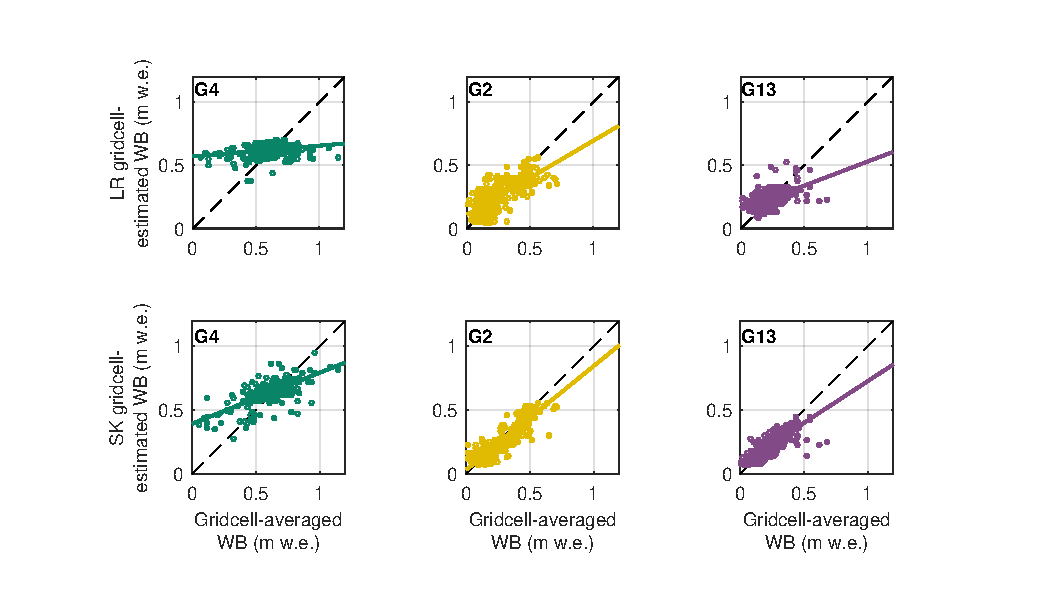
\includegraphics[width =\textwidth]{observedVSestimated_S2.pdf}\\
	\caption{Estimated grid cell SWE found using linear regression (LR) and simple kriging (SK) plotted against observed values of SWE on Glacier 4 (left), Glacier 2 (middle) and Glacier 13 (right). Line of best fit between estimated and observed SWE is also plotted.}
	\label{fig:observedVSestimated_S2}
\end{figure*}

\subsubsection{Linear Regression}

Our sampling design in the LR method ensured that the ranges of topographic parameters covered by the measurements represent more than 70\% of the total area of each glacier (except for the elevation range on Glacier 2, which is 50\%). The analysis of topographic parameters reveals that elevation is the most significant predictor for Glacier 2 and 13, while wind distribution is the most significant predictor for Glacier 4 (Figure \ref{fig:BetaCoeffs}). Elevation, as the predictor, is positively correlated with SWE, meaning that grid cells at higher elevation show higher SWE. While on Glacier 4 wind distribution parameter is negative (i.e. negative correlation with SWE), which indicates less snow in `sheltered' areas, on the other two glaciers wind distribution is positive. Similarly, curvature is positively correlated for Glacier 4 and negatively correlated for the other two glaciers. It is possible that the elevation correlation was accentuated, especially on Glacier 13, during the field campaign due to warmer than normal temperatures and an early (1--2 weeks) start to the melt season (Yukon Snow Survey Bulletin and Water Supply Forecast, May 1, 2016). The southwestern Yukon winter snow pack in 2015 was also well below average, possibly emphasizing effects of early melt onset.

Our mixed insights into dominant predictors of accumulation are consistent with the conflicting results present in the literature. Many winter balance studies have found elevation to be the most significant predictor of SWE \citep[e.g.][]{Machguth2006, McGrath2015}. However, accumulation elevation gradients vary considerably between glaciers \citep[e.g.][]{Winther1998} and other factors, such as
orientation relative to dominant wind direction and glacier shape, have been noted to affect accumulation distribution \citep{Machguth2006,Grabiec2011}.There are also a number of accumulation studies on glaciers that found no significant correlation between accumulation and
topographic parameters and the highly variable snow distribution was attributed to complex local conditions \citep[e.g.][]{Grabiec2011,Lopez2011}.


Wind redistribution and preferential deposition of snow is known to have a large influence on accumulation at sub-basin scales \citep{Dadic2010, Winstral2013}. Our result indicates that wind likely has an impact on snow distribution but that the wind redistribution parameter may not adequately represent this impact. For example, Glacier 4 is located in a curved valley with steep side walls so having a single cardinal direction for wind may be inappropriate. Further, the scale of deposition may be smaller than the resolution of the Sx parameter estimated from our DEM. Our results corroborate \cite{McGrath2015}, who completed a winter balance study on six Alaskan glaciers (DEM resolutions of 5 m) and found that Sx was the only other significant parameter, besides elevation, for all glaciers. Regression coefficients were small ($\<$ 0.3) and in some cases, negative. Sublimation from blowing snow has also been shown to be an important mass loss from ridges  \citep{Musselman2015}. Incorporating snow loss as well as redistribution and preferential deposition may be needed for accurate representations of seasonal accumulation.

Since we are unable to measure SWE in grid cells that have high topographic parameter values, we
must extrapolate relationships linearly. The accumulation area, where there are few observations, is most susceptible to extrapolation errors (Figure \ref{fig:LR_SK_map}). This area typically also has the highest SWE values, affecting the specific winter balance estimated for the glacier. In our study, the dependence of SWE on elevation, especially on Glacier 2, means that LR extrapolation results in almost 2 m w.e. estimated in the parts of the accumulation area. This exceptionally large estimate of SWE is unlikely for a continental snow pack. Extrapolating a LR that is fitted to predominantly ablation area SWE values is likely erroneous.

While a LR can be used to predict distributed SWE in other basins, we found that transfer of LR coefficients between glaciers results in large estimation error. The lowest overall RMSE (0.2051 m w.e.) results from calculating a LR using all available observations. Our results are consistent with \cite{Grunewald2013}, who found that local statistical models are able to perform well but they cannot be transferred to different regions and that regional-scale models are not able to explain the majority of variance. The inter-basin variability in our study range is greater than the intra-basin variability.

\subsubsection{Simple kriging}

For all study glaciers, simple kriging (SK) is a better predictor of observed SWE than LR (Figure  \ref{fig:LR_SK_map}). However, the winter balance uncertainty that arises from using SK is large, and unrealistic values of 0 m w.e. winter balance can be estimated. Our observations are generally limited to the ablation area so SK estimates an almost uniform distribution of SWE in the accumulation areas of the study glaciers, which is inconsistent with observations described in the literature \citep[e.g.][]{Machguth2006, Grabiec2011}. Extrapolation using SK leads to large uncertainty in estimating winter balance, which further emphasis the need for SWE observations in the accumulation area.

SK cannot be used to understand physical processes that may be controlling snow distribution and cannot be used to estimate accumulation beyond the study area. However, fitted kriging parameters, including the nugget and spatial correlation length, can provide insight into important scales of variability. Glaciers 2 and 13 have long correlation lengths and small nuggets indicating variability at large scales (see Supplementary Material Table \ref{tab:range&nugget}). Conversely, Glacier 4 has a short correlation length and large nugget, indicating that accumulation variability occurs at small scales.

\begin{figure}
	\centering
	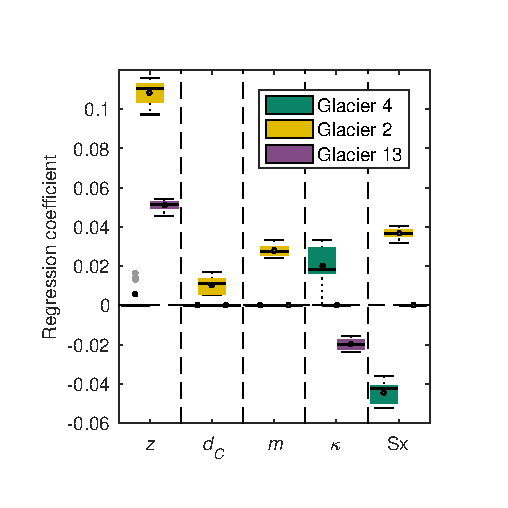
\includegraphics[width =0.5\textwidth]{BetaCoeffs.pdf}\\
	\caption{Distribution of regression coefficients for linear regression of grid cell topographic parameters and SWE calculated using eight density options on study glaciers. Topographic parameters include elevation ($z$), distance from centreline ($d_C$), slope ($m$) , curvature ($\kappa$), and wind exposure (Sx). Regression coefficients that were not significant were assigned a value of zero. Aspect and ``northeness'' are not shown because coefficient values are zero for all glaciers. Outlier values are shown as gray dots.}
	\label{fig:BetaCoeffs}
\end{figure}

\begin{figure*}
	\centering
	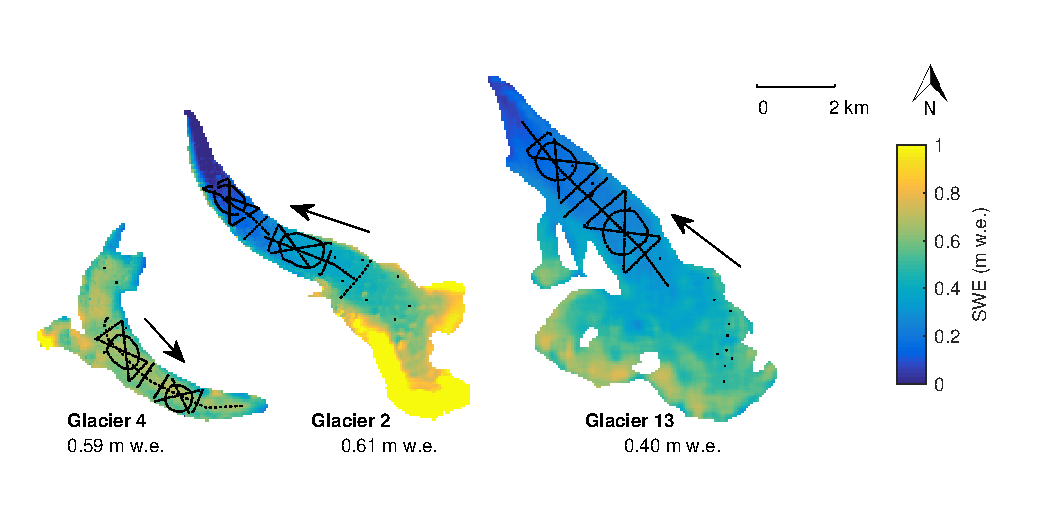
\includegraphics[width =\textwidth]{LR_map.pdf}\\
		\vspace{-16 mm}
    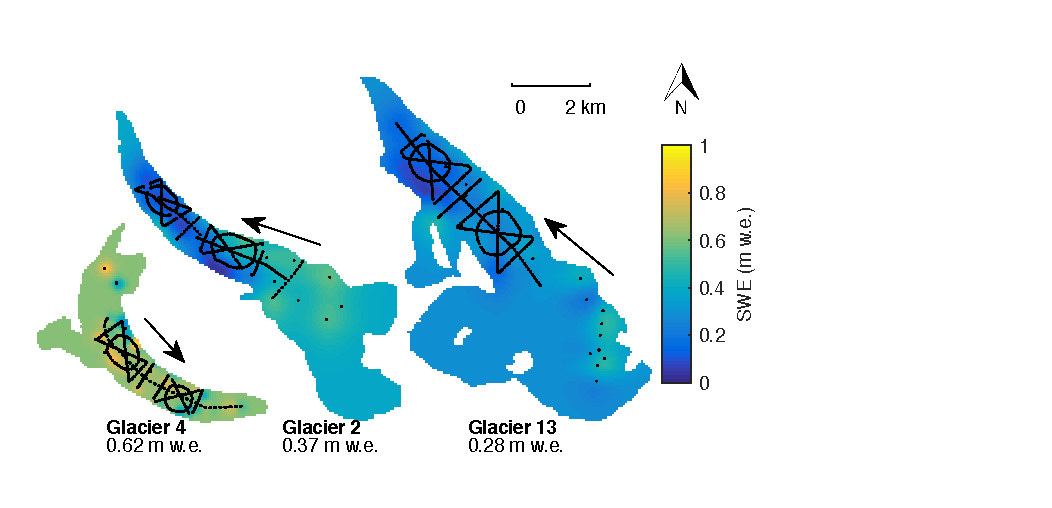
\includegraphics[width =\textwidth]{SK_map.pdf}\\
	\caption{Spatial distribution of SWE estimated using linear regression (upper) and simple kriging (lower). Grid-cell SWE observations are found using glacier wide mean snow pit density and are shown as black dots. Glacier flow directions are indicated by arrows. Specific winter balance values are also shown.}
	\label{fig:LR_SK_map}
\end{figure*}



\subsection{Uncertainty analysis}

Specific winter balance is affected by uncertainty introduced when interpolating density ($\sigma_{\rho}$), when calculating grid cell SWE values ($\sigma_{\mathrm{SWE}}), and when interpolating observations ($\sigma_{\mathrm{INT}}$). We find that when using LR and SK, interpolation uncertainty has a larger effect on winter balance uncertainty than density uncertainty or SWE uncertainty. The probability density function (PDF) that arises from SWE uncertainty is much narrower than the PDF that arises from interpolation uncertainty (Figure \ref{fig:WSMBDist_LR} and Table \ref{tab:WSMBdistribution_sigma}).

 \begin{table}[]
\centering
\caption{Standard deviation ([$\times10^{-2}$ m w.e.]) of winter balance distributions arising from SWE ($\sigma_{\mathrm{SWE}}$), density ($\sigma_{\rho}$) and interpolation ($\sigma_{\mathrm{INT}}$) uncertainty. Result for Glacier 4 (G4), Glacier 2 (G2) and Glacier 13 (G13) are shown.}
\label{tab:WSMBdistribution_sigma}
\begin{tabular}{ccccccc}
\textbf{} & \multicolumn{3}{c}{\textbf{Linear Regression}} & \multicolumn{3}{c}{\textbf{Simple Kriging}} \\
 & $\sigma_{\rho}$ & $\sigma_{\mathrm{SWE}}$ & $\sigma_{INT}$ & $\sigma_{\rho}$ & $\sigma_{\mathrm{SWE}}$ & $\sigma_{\mathrm{INT}}$ \\
\midrule
\textbf{G4} & 1.90 & 0.86 & 2.13 & 2.15 & 0.85 & 14.05 \\
\textbf{G2} &3.37 & 1.80 & 3.09 & 2.03 & 2.53 & 13.78 \\
\textbf{G13} & 1.68 & 1.12 & 2.80 & 1.27 & 1.15 & 9.65
\end{tabular}
\end{table}

\begin{figure*}
	\centering
\hspace*{-1.2cm}
	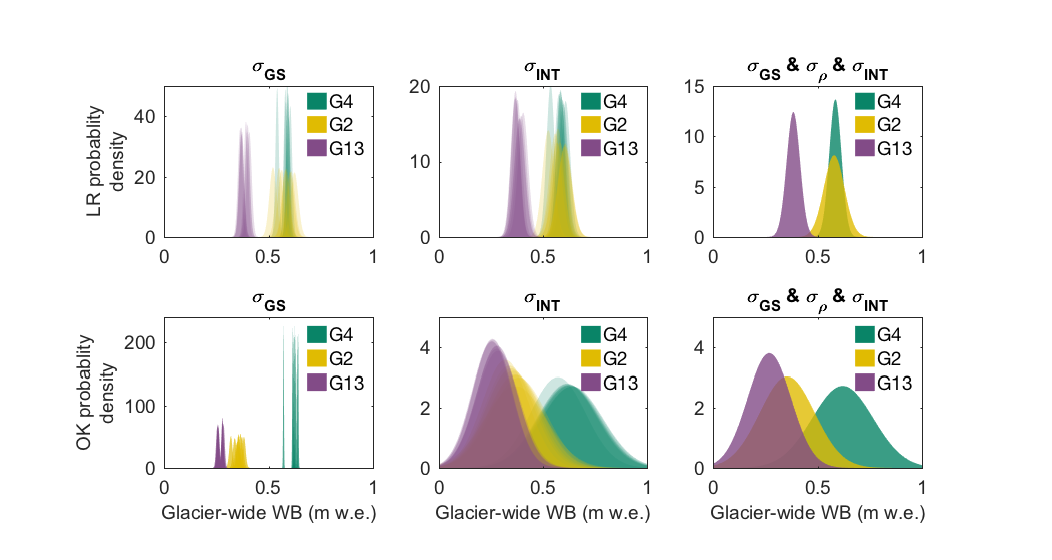
\includegraphics[width =1.1\textwidth]{WSMBDist.pdf}\\
	\caption{Probability density functions (PDFs) fitted to distributions of specific winter balance values that arise from (left) SWE uncertainty ($\sigma_{SWE}$), (middle) interpolation uncertainty ($\sigma_{INT}$) and (right) all three sources of uncertainty. Results from a linear regression interpolation (top panels) and simple kriging (bottom panels) are shown. Each PDF is calculated using one of eight density interpolation methods for Glacier 4 (G4), Glacier 2 (G2) and Glacier 13 (G13).}
	\label{fig:WSMBDist_LR}
\end{figure*}

A large contributor to uncertainty arises from extrapolation beyond the sampled region, which results in high uncertainty in estimated SWE in the accumulation area. The winter balance distributions obtained using LR and SK overlap for each glacier but the distribution modes differ, with SK generally estimating lower winter balance in the accumulation area, which lowers the overall winter balance estimate. It is important to note that although the distributions from LR are narrower than those from SK, that does not necessitate that LR is a more accurate method of estimating winter balance. Based on the sources of uncertainty chosen, LR appears to be more precise than SK but the methods of calculating interpolation uncertainty are different so the distributions should not be directly compared.

SWE uncertainty is the smallest contributor to winter balance uncertainty. Therefore, obtaining the most accurate value of SWE to represent a grid cell, even a relatively large grid cell, does not need to be a priority when designing a snow survey. Many parts of a glacier are characterized by a relatively smooth surface, with roughness lengths on the order of centimetres \citep{Hock2005} resulting in low snow depth uncertainty. However, we assume that the sampled grid cells are representative of the uncertainty across the entire glacier, which is likely not true for areas with debris cover, crevasses and steep slopes.

Density, SWE, and interpolation uncertainty all contribute to spatial patterns of winter balance uncertainty (Figure \ref{fig:WSMBspatialvar}).  For both LR and SK, the greatest uncertainty in estimated SWE occurs in the accumulation area. When LR is used, estimated SWE is highly sensitive to the elevation regression parameter. In the case of SK, uncertainty is greatest in areas far from observed SWE, which consist of the upper accumulation area on Glaciers 2 and 13. uncertainty is greatest on Glacier 4 when LR interpolation is used at the upper edges of the accumulation area, which correspond to the locations with extreme values of the wind redistribution parameter. When SK is used for interpolation on Glacier 4, uncertainty is greatest at the measured grid cells, which highlights the short correlation length and the large effect of density interpolation on the SK accumulation estimate.

Using a Monte Carlo experiment to propagate uncertainty allowed us to quantify effects of uncertainty on estimates of winter balance. However, our analysis did not include uncertainty arising from a number of data sources, which we assumed to contribute negligibly to the uncertainty in winter balance or to be encompassed by investigated sources of uncertainty. These sources of uncertainty include error associated with SP and FS density measurement, DEM vertical and horizontal error and error associated with estimating measurement locations.

\begin{figure*}
	\centering
	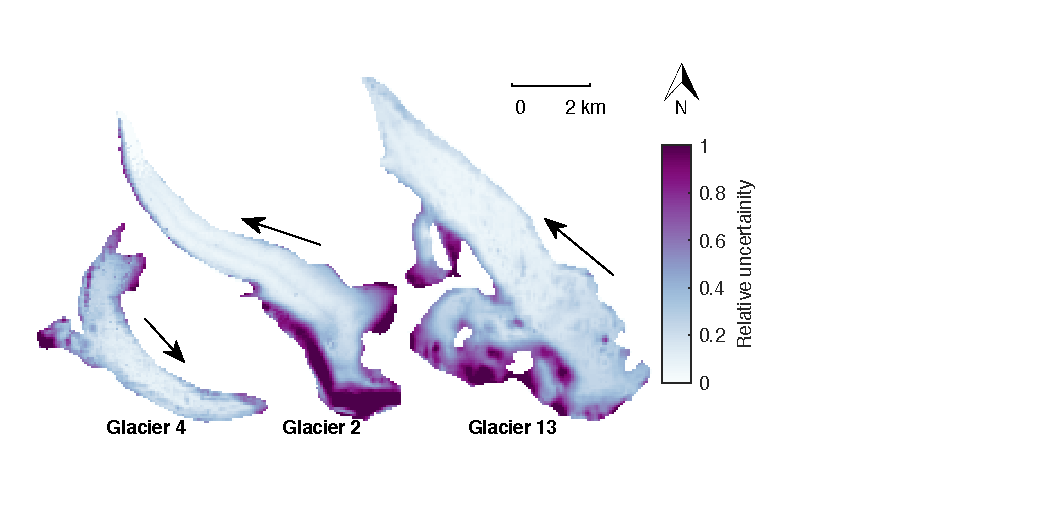
\includegraphics[width =\textwidth]{SpatialVar_LR.pdf}\\
	\vspace{-20 mm}
	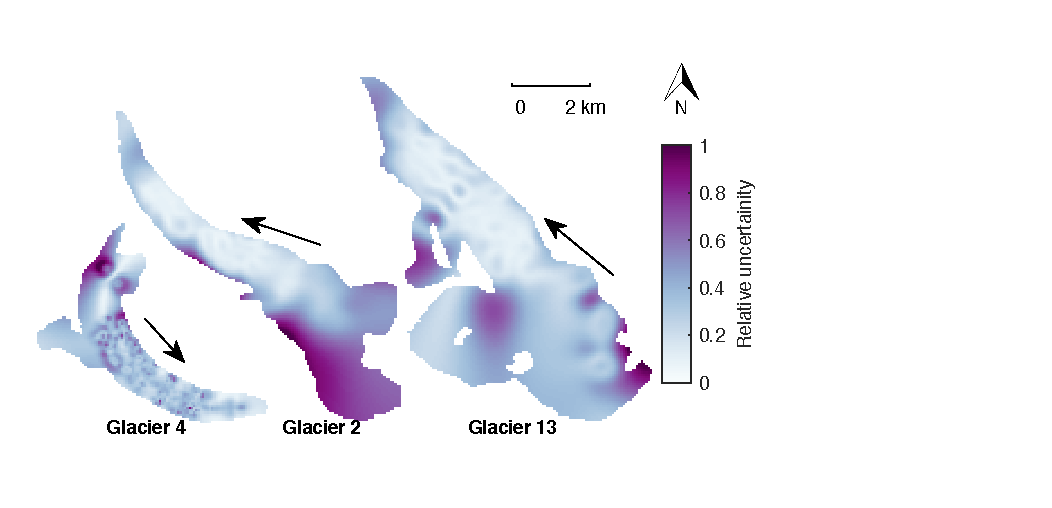
\includegraphics[width =\textwidth]{SpatialVar_SK.pdf}\\
	\caption{Uncertainty of SWE estimated using linear regression (top) and simple kriging (bottom). Uncertainty is a relative quantity measured by taking the sum of differences between one hundred estimates of distributed winter balance that include SWE uncertainty and, in the case of linear regression, regression uncertainty. The sum is then normalized for each glacier. Glacier flow directions are indicated by arrows.}
	\label{fig:WSMBspatialvar}
\end{figure*}


\subsection{Mountain range accumulation gradient}

An accumulation gradient is observed for the continental side of the St. Elias Mountains (Figure \ref{fig:AccumGrad}). Accumulation data are compiled from \cite{Taylor1969}, the three glaciers presented in this paper, as well as two snow pits we dug near the head of the Kaskawalsh Glacier in May 2016. The data show a linear decrease in observed SWE as distance from the main mountain divide (identified by \cite{Taylor1969}) increases, with a gradient of $-0.024$ m w.e. km$^{-1}$. While the three study glaciers fit the regional relationship, the same relationship would not apply when just the Donjek Range is considered. Therefore, glacier location within a mountain range also affects glacier-wide winter balance. Interaction between meso-scale weather patterns and mountain topography is a major driver of glacier-wide accumulation. Further insight into mountain-scale accumulation trends can be achieved by investigating moisture source trajectories and orographic precipitation contribution to accumulation. 

\begin{figure}
	\centering
	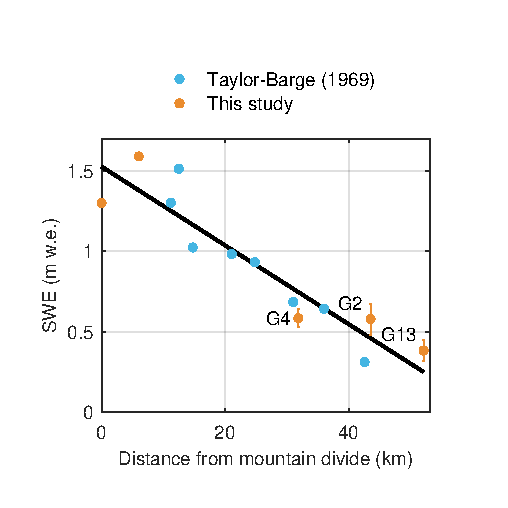
\includegraphics[width =0.5\textwidth]{AccumGrad.pdf}\\
	\caption{Relation between SWE and linear distance from St. Elias mountain divide, located at the head of the Kaskawalsh Glacier. Blue dots are snow pit derived SWE values from \cite{Taylor1969}. Orange dots furthest from the divide are mean winter balance from Glaciers 4, 2 and 13, with 95\% confidence interval using a linear regression interpolation. Orange dots close to the divide are snow pit derived SWE value at two locations in the accumulation area of the Kaskawalsh Glacier collect in May 2016. Black line indicates line of best fit (R$^2=0.85$).}
	\label{fig:AccumGrad}
\end{figure}


\subsection{Limitations and future work}

Extensions to this work could include an investigation of experimental design, examining the effects of DEM grid size on winter balance and resolving temporal variability. Our sampling design was chosen to extensively sample the ablation area and is likely too finely resolved for many future mass balance surveys to replicate. Determining a sampling design that minimizes error and reduces the number of measurements, known as data efficiency thresholds, would contribute to optimizing snow surveys in mountainous regions. For example, \cite{Lopez2010} concluded that $200-400$ observations are needed to obtain accurate and robust snow distribution models. 

DEM grid cell size is known to significantly affect computed topographic parameters and the ability for a DEM to resolve important hydrological features (i.e. drainage pathways) in the landscape \citep{Zhang1994, Garbrecht1994, Guo-an2001, Lopez2010}, which can have implications for calculating a LR that uses topographic parameters.  \cite{Zhang1994} found that a 10 m grid cell size is an optimal compromise between increasing resolution and large data volumes. Further, the importance of topographic parameters in predicting SWE is correlated with DEM grid size \citep[e.g.][]{Kienzle2004, Lopez2010}. A decrease in spatial resolution of the DEM results in a decrease in the importance of curvature and an increase in the importance of elevation. A detailed and ground controlled DEM is therefore needed to identify the features that drive accumulation variability. Even with a high resolution DEM, microtopography that creates small scale snow variability cannot be resolved. For example, the lower part of Glacier 2 has an undulating ice surface (on the order of 5 m horizontal and 0.5 m vertical) that results in large variability in snow depth.

Temporal variability in accumulation is not considered in our study. While this limits the extent of our conclusions, a number of studies have found temporal stability in spatial patterns of snow accumulation and that terrain-based model could be applied reliable between years \citep[e.g.][]{Grunewald2013}. For example, \cite{Walmsley2015} analyzed more than 40 years of accumulation recorded on two Norwegian glaciers and found that snow accumulation is spatially heterogeneous yet exhibits robust time stability in its distribution. 

%%%%%%%%%%%%%%%%%%%%%%%%%%%%%%%%%%
% CONCLUSION
%%%%%%%%%%%%%%%%%%%%%%%%%%%%%%%%%%
\section{Conclusion}

We estimate spatial accumulation patterns and specific winter balance for three glaciers (labelled as Glacier 2, Glacier 4 and Glacier 13) in the St. Elias mountains from extensive snow depth and density sampling. Our objectives are to (1) examine methods and uncertainties when moving from snow measurements to estimating winter balance and (2) show how snow variability, data error and our methodological choices interact to create uncertainty in our estimate of winter balance.

We find that the method used to interpolate observations has a large effect on winter balance estimates and its associated uncertainty. On Glacier 4, winter balance estimates are consistent between linear regression (LR) and simple kriging (SK) but both explain only a small portion of observed variance, highlighting that although the winter balance estimates are relatively precise they may not necessarily be accurate. On Glaciers 2 and 13, LR and SK are better able to estimate observed SWE values but winter balance estimates differ considerably between the two interpolation methods due to extrapolation into the accumulation area. SK is a non-parametric interpolation method that relies heavily on regular and dense sampling so extrapolation is sensitive to marginal data values and the data mean. LR employs parameters that act as proxies for physical processes, which provides insight into drivers of SWE distribution, constrains extrapolation values and can be spatially transferred. It is therefore critical that future winter balance studies report which interpolation method is used to estimate winter balance, the ability for the model to estimate observed measurements and the uncertainty that results from fitting the interpolation model. 

For our study glaciers, the total winter balance uncertainty ranges from 0.03 (8\%) to 0.15 (54\%) m w.e. depending primarily on the interpolation method. The smallest winter balance uncertainty source is the representation of grid cell SWE. Future studies could reduce winter balance uncertainty by increasing the spatial distribution of snow depth sampling rather than obtaining many measurements within a single grid cell. In our work, increased sampling within the accumulation area would better constrain SWE extrapolation and decrease uncertainty. Our results indicate that using extrapolated data to compare with winter balance estimates from remote sensing or modelling studies may produce misleading results. If possible, comparison studies should use observed SWE data rather than interpolated winter balance values. 

Snow distribution patterns are found to differ considerably between glaciers, highlighting strong intra- and inter-basin variability and accumulation drivers acting on multiple scales. SWE distribution on Glacier 4 is highly variable, as indicated by shorter range distance, higher nugget value and lower explained variance. Glaciers 2 and 13 have lower SWE variability and elevation is the primary control of observed variation. Despite challenges in accurately estimating winter balance, our data are consistent with a previously reported linear decrease in SWE with increased distance from the main topographic divide along the continental side of the St. Elias Mountains. This trend indicates that glacier location within a mountain range has a large influence on winter balance. 

%----------------------------------------------------------------------------------------
%	REFERENCE LIST
%----------------------------------------------------------------------------------------
%
\bibliography{/home/glaciology1/Documents/MastersDocuments/MastersLit}
%\bibliography{/Users/Alexandra/Documents/SFU/MastersDocuments/MastersLit}
\bibliographystyle{igs}

%----------------------------------------------------------------------------------------
\pagebreak 
\section{Supplementary material}

%% TOPO DETAILS
\begin{table*}[!htbp]
\centering%
\caption{Description of topographic parameters used in the linear regression.}
\label{tab:TopoParams}
\begin{tabularx}{\linewidth}{XXXXX}
\midrule
\textbf{\begin{tabular}[c]{@{}l@{}}Topographic\\ parameter\end{tabular}} & \textbf{Definition} & \textbf{\begin{tabular}[c]{@{}l@{}}Calculation \\ method\end{tabular}} & \textbf{Notes} & \textbf{Source} \\ \midrule
\textbf{Elevation ($z$)} &  & Values taken directly from DEM &  &  \\
\textbf{Distance from centreline ($d_C$)} &  & Minimum distance between the Easting and Northing of the northwest corner of each grid cell and a manually defined centreline &  &  \\
\textbf{Slope ($m$)} & Angle between a plane tangential to the surface (gradient) and the horizontal & \texttt{r.slope.aspect} module in GRASS GIS software run through QGIS &  & \cite{Mitavsova1993, Hofierka2009, Olaya2009} \\
\textbf{Aspect ($\alpha$)} & Dip direction of the slope & \texttt{r.slope.aspect} module in GRASS GIS software run through QGIS & $\sin(\alpha)$, a linear quantity describing a slope as north/south facing, is used in the regression & \cite{Mitavsova1993, Hofierka2009, Olaya2009} \\
\textbf{Mean curvature ($\kappa$)} & Average of profile (direction of the surface gradient) and tangential curvature (direction of the contour tangent) & \texttt{r.slope.aspect} module in GRASS GIS software run through QGIS & mean-concave (positive values) terrain with relative accumulation and mean-convex (negative values) terrain with relative scouring & \cite{Mitavsova1993, Hofierka2009, Olaya2009} \\
\textbf{``Northness'' ($N$)} & $-1$ represents a vertical, south facing slope, a value of $+1$ represents a vertical, north facing slope, and a flat surface yields 0 & Product of the cosine of aspect and sine of slope &  & \cite{Molotch2005} \\
\textbf{Wind exposure/shelter parameter (Sx)} &  & Executable obtained from Adam Winstral that follows the procedure outlined in \cite{Winstral2002} & Calculation based on selecting a cell within a certain angle and distance from the cell of interest that has the greatest upward slope relative to the cell of interest & \cite{Winstral2002}
\end{tabularx}
\end{table*}

%% TOPO SAMPLED VS FULL
\begin{figure*}
	\centering
	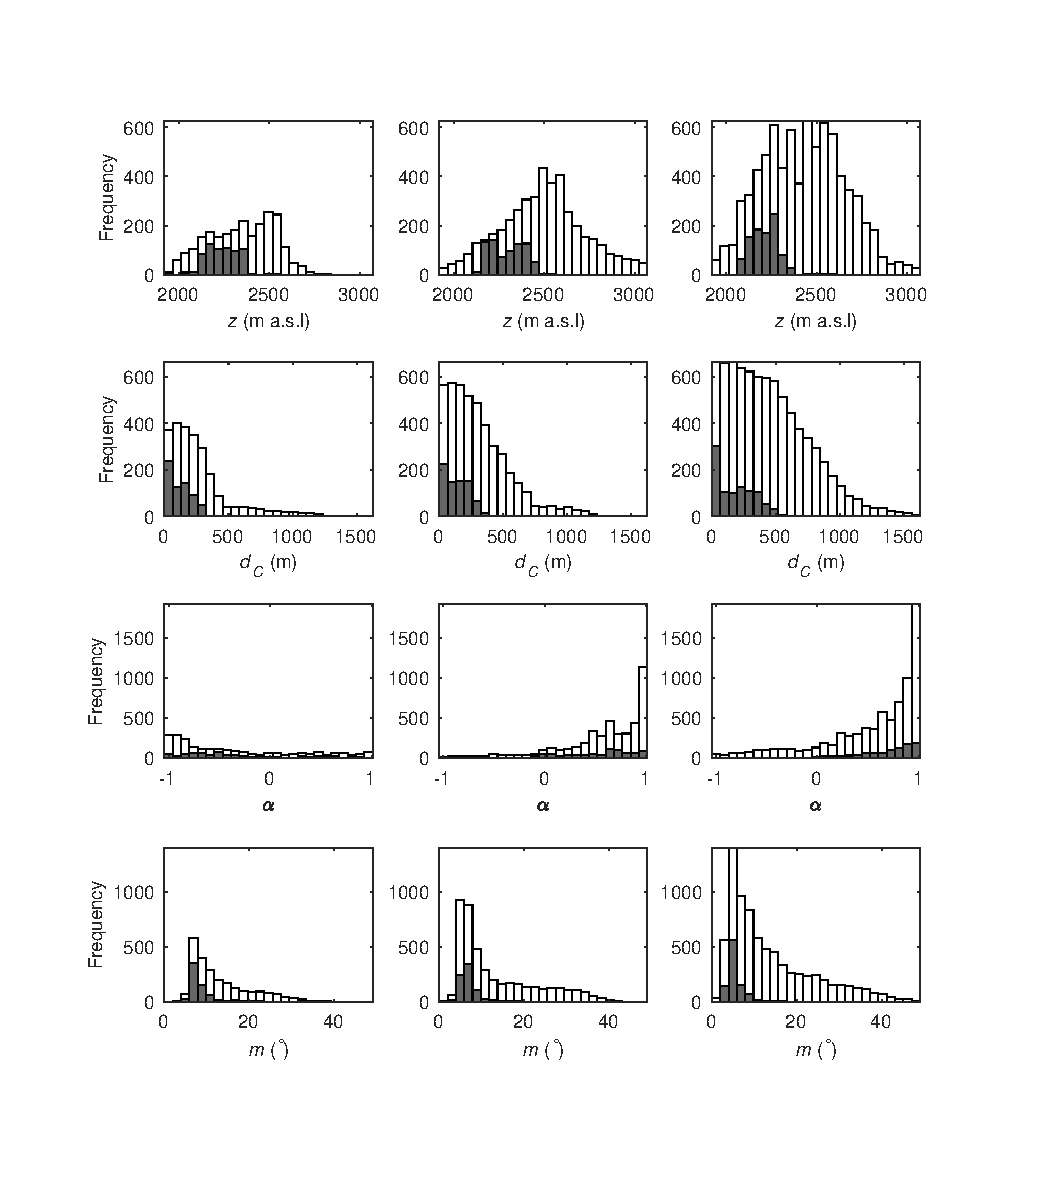
\includegraphics[width =\textwidth]{TopoParamsSampled1.pdf}\\
	\caption{Distribution of topographic parameters over Glacier 4 (left), Glacier 2 (middle) and Glacier 13 (right) are shown in white. Distribution of topographic parameter values from sampled grid cells in shown in gray. Topographic parameters include elevation ($z$), distance from centreline ($d_C$), aspect ($\alpha$), slope ($m$), northness ($N$), mean curvature ($\kappa$), and winter redistribution (Sx).}
	\label{fig:TopoParamsSampled1}
\end{figure*}
\begin{figure*}
	\centering
	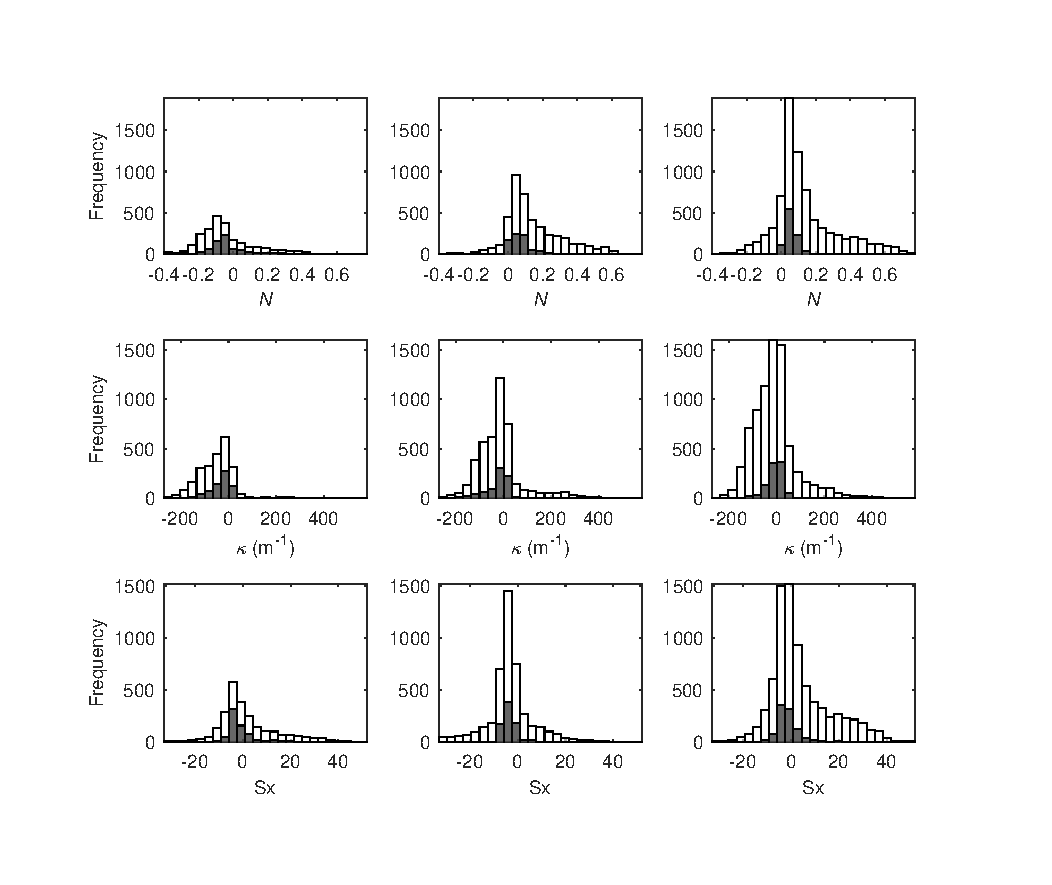
\includegraphics[width =\textwidth]{TopoParamsSampled2.pdf}\\
	\caption{See Figure \ref{fig:TopoParamsSampled1}}
	\label{fig:TopoParamsSampled2}
\end{figure*}

%% DENSITY VALUES USED

\begin{table}[]
\centering
\caption{Snow density values used for interpolating density based on snow pit (SP) densities and Federal Sampler (FS) densities. Four interpolation methods are chosen: (1) using a mean snow density for all three glaciers (Range mean density), (2) using a mean density for each glacier (Glacier mean density), (3) using a regression between density and elevation (Elevation regression), and (4) inverse-distance weighted mean density (not shown).}
\label{tab:Density}
\begin{tabular}{cccc}
 &  & \textbf{\begin{tabular}[c]{@{}c@{}}SP density\\ (kg m$^{-3}$)\end{tabular}} & \textbf{\begin{tabular}[c]{@{}c@{}}FS density\\ (kg m$^{-3}$)\end{tabular}} \\
 \midrule
\textbf{\begin{tabular}[c]{@{}c@{}}Range \\ mean density\end{tabular}} &  & 342 & 316 \\
\midrule
\multirow{3}{*}{\textbf{\begin{tabular}[c]{@{}c@{}}Glacier\\ mean density\end{tabular}}} & G4 & 348 & 327 \\
 & G2 & 333 & 326 \\
 & G13 & 349 & 307 \\
 \midrule
\multirow{3}{*}{\textbf{\begin{tabular}[c]{@{}c@{}}Elevation \\ regression\end{tabular}}} & G4 & $0.03z+274$ & $-0.16z+714$ \\
 & G2 & $-0.14z+659$ & $0.24z-282$ \\
 & G13 & $-0.20z+802$ & $0.12z+33$
\end{tabular}
\end{table}

%% TOPOGRAPHIC PARAMETERS EXPLAINED
\subsubsection{Topographic parameters}

First, cross-validation is used to obtain a set of $\beta_i$ values that have greater predictive ability. We select 1000 random subsets (2/3 values) of the data to fit the LR and the remaining data (1/3 values) are used to calculate a root mean squared error (RMSE) \citep{Kohavi1995}. Regression coefficients resulting in the lowest RMSE are selected. Second, we use model averaging to take into account uncertainty when selecting predictors and to also maximize predictive ability \citep{Madigan1994}. Models are generated by calculating a set of $\beta_i$ for all possible combinations of predictors. Following a Bayesian framework, model averaging involves weighting all models by their posterior model probabilities \citep{Raftery1997}. To obtain the final regression coefficients, the $\beta_i$ values from each model are weighted according to the relative predictive success of the model, as assessed by the Bayesian Information Criterion (BIC) value \citep{Burnham2004}. BIC penalizes more complex models, which further reduces the risk of overfitting.

Topographic parameters are easy to calculate proxies for physical processes, such as orographic precipitation, solar radiation effects, wind redistribution and preferential deposition. We derive all parameters (Table \ref{tab:TopoParams}) for our study from a SPOT-5 DEM ($40\times40$ m) \citep{Korona2009}. Two DEMs are stitched together to encompass the Donjek Range. An iterative 3D-coregistration algorithm \citep{Berthier2007} is used to correct the horizontal ($\sim$2 m E, $\sim$4 m N) and vertical (5.4 m) discrepancy between the two DEMs before stitching. 

Visual inspection of the curvature fields calculated using the full DEM shows a noisy spatial distribution that did not vary smoothly. To smooth the DEM, various smoothing algorithms and window sizes are applied and the combination that produces the highest correlation between topographic parameters and SWE is chosen. Inverse-distance weighted, Gaussian and grid cell averaging smoothing all with window sizes of 3$\times$3, 5$\times$5, 7$\times$7 and 9$\times$9 are used. Grid cell average smoothing with a 7$\times$7 window resulted in the highest overall correlation between curvature (second derivative) and SWE as well as slope (first derivative) and SWE. We use the smoothed DEM to calculate curvature, slope, aspect and ``northness''.

%% RANGE AND NUGGET VALUES
\begin{table}[]
\centering
\caption{Range and nugget values for simple kriging interpolation}
\label{tab:range&nugget}
\begin{tabular}{ccc}
\midrule
 & \textbf{\begin{tabular}[c]{@{}c@{}}Range \\ (m)\end{tabular}} & \textbf{\begin{tabular}[c]{@{}c@{}}Nugget \\ ($\times10^3$m w.e.)\end{tabular}} \\ \midrule
\textbf{G4} & 90 & 10.5 \\
\textbf{G2} & 404 & 3.6 \\
\textbf{G13} & 444 & 4.8
\end{tabular}
\end{table}

\end{document}